\documentclass{beamer}
\usetheme{Madrid}

\title{Question Answering in the Biomedical Domain}
\author{Vincent Nguyen, Sarvnaz Karimi, Zhenchang Xing}
\centering

\begin{document}
\maketitle

\begin{frame}{Motivation}
\framesubtitle{Why is this important?}
\begin{itemize}
\end{itemize}
\vspace{0.2cm}
\vspace*{3cm}
\end{frame}
\begin{frame}{Stats}
\begin{itemize}
\end{itemize}
\end{frame}

\begin{frame}{Challenges?}
\framesubtitle{How do we overcome them?}
\begin{itemize}
\end{itemize}
\end{frame}

\begin{frame}{}
\framesubtitle{}
 
\end{frame}

\begin{frame}{Question Hierarchy}
  \framesubtitle{Phrase-level}
  
  \begin{itemize}
      \item Apply a 1-D Convolution with unigram, bigram and trigram filters over Word Embeddings, $q^w_t \in Q^w$.
  \end{itemize}
  
  \begin{equation*}
      \mathbf{\hat{q}}^p_{s,t} = \tanh(\mathbf{W}^s_c \mathbf{q}^w_{t:t+s-1}), s \in \{1,2,3\}
  \end{equation*}
  
  \begin{itemize}
      \item At each word location, $q_t \in Q$, apply a max-pooling operation to obtain phrase-level features
  \end{itemize}
  
  \begin{equation*}
      \mathbf{{q}}^p_{t} = \max(\mathbf{\hat{q}}^p_{1, t}, \mathbf{\hat{q}}^p_{2, t},\mathbf{\hat{q}}^p_{3, t}), t \in \{1, 2, ... T\}
  \end{equation*}
  
  \begin{itemize}
      \item This pooling approach adaptively selects the most suitable n-gram feature at each time-step while preserving sequence length and word order.
  \end{itemize}
\end{frame}

\begin{frame}{Question Hierarchy}
  \framesubtitle{Sentence-level}  
  
  \begin{itemize}
      \item Use an LSTM to encode the sequence $\mathbf{q}^p_t$ after the max-pooling operation over the unigram, bigram and trigram features
  \end{itemize}
  
  \begin{equation*}
      \mathbf{q}^s_t = \text{LSTM}(\mathbf{q}^p_t)
  \end{equation*}

\end{frame}

\begin{frame}{Hierarchy}
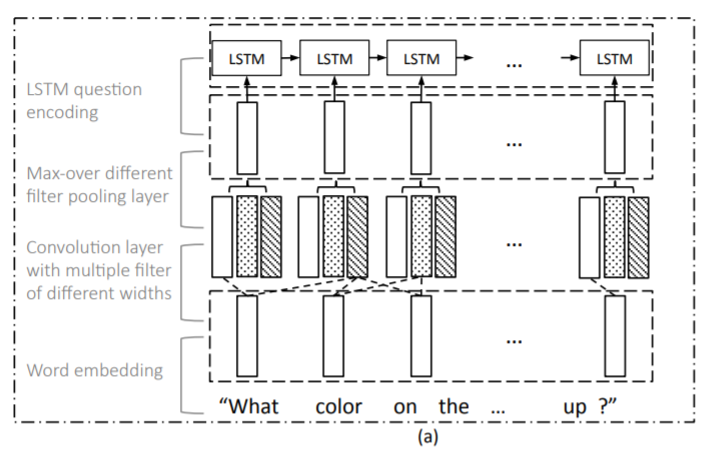
\includegraphics[width=12.2cm]{Annotation 2020-02-09 152111.png}
\end{frame}

\begin{frame}{Key Ideas}
\begin{itemize}
\item \color{gray} Question Hierarchy
\begin{itemize}
    \item \color{gray} Word-level
    \item Phrase-level
    \item Sentence-level
\end{itemize}
\item \color{black} Co-Attention for VQA
\begin{itemize}
    \item Parallel 
    \item \color{black} Alternating 
\end{itemize}
\end{itemize}
\end{frame}

\begin{frame}{Parallel Co-Attention}
\begin{enumerate}
    \item Generate an affinity matrix that connects the image, $\matbf{V}$, and question, $\mathbf{Q}$, at all image-locations and question-locations at each level in the hierarchy
\end{enumerate}

\begin{equation*}
    \mathbf{C} = \tanh(\mathbf{Q}^T\mathbf{W}_b\mathbf{V})
\end{equation*}

\begin{enumerate}[2]
    \item Use this affinity matrix as a feature to predict image and question maps 
    \item The affinity matrix acts as an attention space transformer (question projects to image and vice versa)
\end{enumerate}

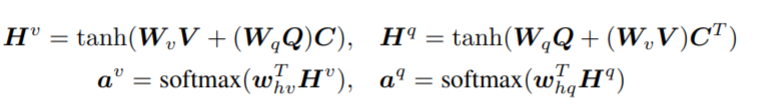
\includegraphics[width=8.5cm]{Annotation 2020-02-09 153558.png}
\end{frame}

\begin{frame}{Diagram}
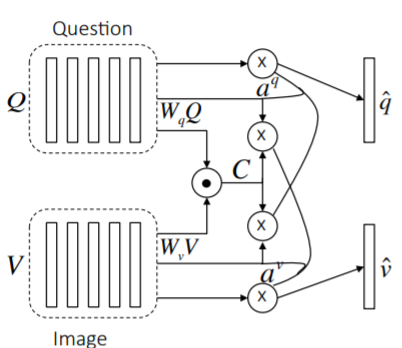
\includegraphics[width=8cm]{Annotation 2020-02-10 111151.png}
\end{frame}

\begin{frame}{Alternating Co-Attention}
\begin{itemize}
    \item Sequentially alternate between generating image and question attention
    \begin{enumerate}
        \item Summarise the question into a single vector
        \item Attend to the image based on the question vector
        \item Attend to the question based on the attended image feature
    \end{enumerate}
\end{itemize}

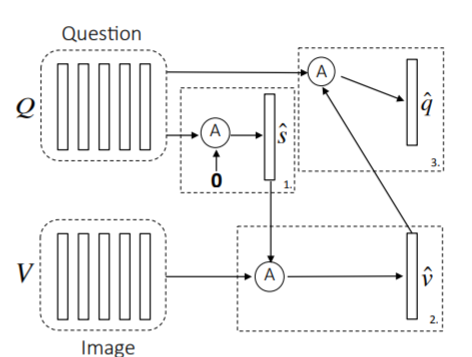
\includegraphics[width=7.5cm]{Annotation 2020-02-10 111002.png}

\end{frame}

\begin{frame}{Full Model}
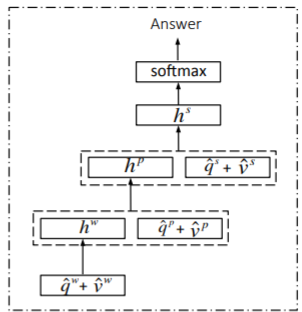
\includegraphics[]{Annotation 2020-02-10 113904.png}
\end{frame}

\begin{frame}{Ablation}
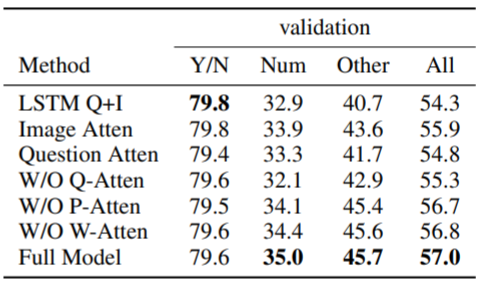
\includegraphics[]{Annotation 2020-02-10 111716.png}
\end{frame}

\begin{frame}{Attention Maps}
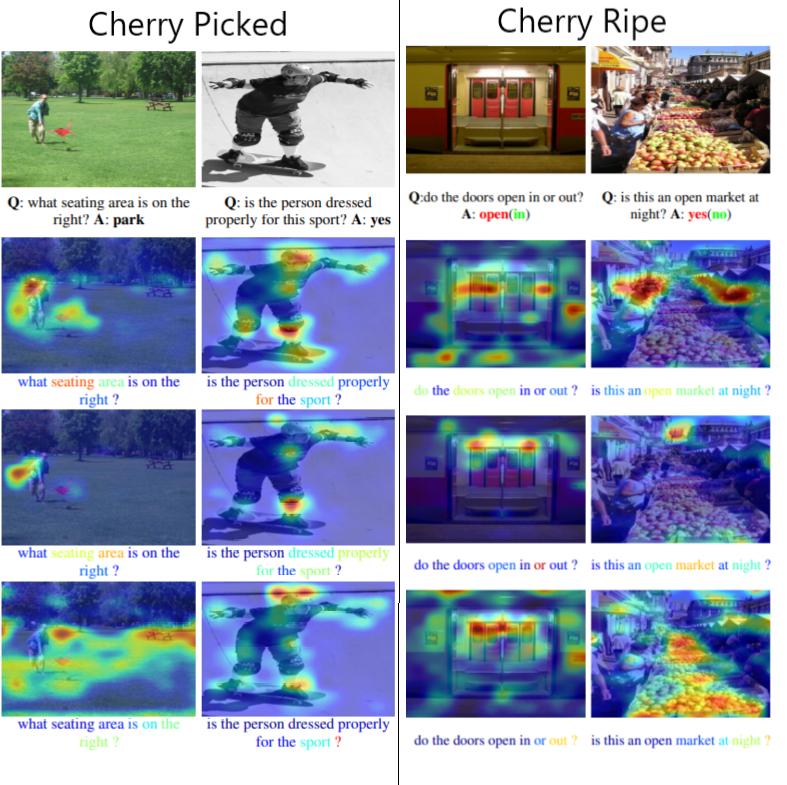
\includegraphics[width=8.2cm]{Annotation 2020-02-10 113657.png} 
\end{frame}

\begin{frame}{Demo}

\url{http://vqa.cloudcv.org/}
    
\end{frame}

\end{document}
